\chapter{Results}
\label{chap:results}
This Chapter illustrates the results of the data exploration and the statistical analysis. First, we describe the retrieved data on a user level in \autoref{sec:res_users}. Next, we look at the repository characteristics, including all metrics and details about license, language, and topic usage in \autoref{sec:res_repos}. This is followed by inspecting the \acrshort{fair} variables in more detail in \autoref{sec:res_fair}. Lastly, we look at the statistical analysis of the dataset, which includes the statistical tests in \autoref{sec:stattests} and the classification of research software against non-research software in \autoref{sec:classification}.

\section{Users characteristics}
\label{sec:res_users}
The number of collected users per faculty can be seen in \autoref{fig:user_count}. \textit{UtrechtUniversity} represents the GitHub repositories of the organizational user \textit{UtrechtUniversity}. \autoref{fig:user_count} shows no users within the collected data from the \textit{Faculty of Medicine}. It is expected to have no users related to the Faculty of Medicine as they are employed by the \acrshort{umcu} and, therefore, not part of this study. It is also expected that the \textit{Faculty of Science} would have the highest number of users, as they are most likely to extensively use GitHub for research and non-research purposes. 

\begin{figure}[h!]
\centerline{
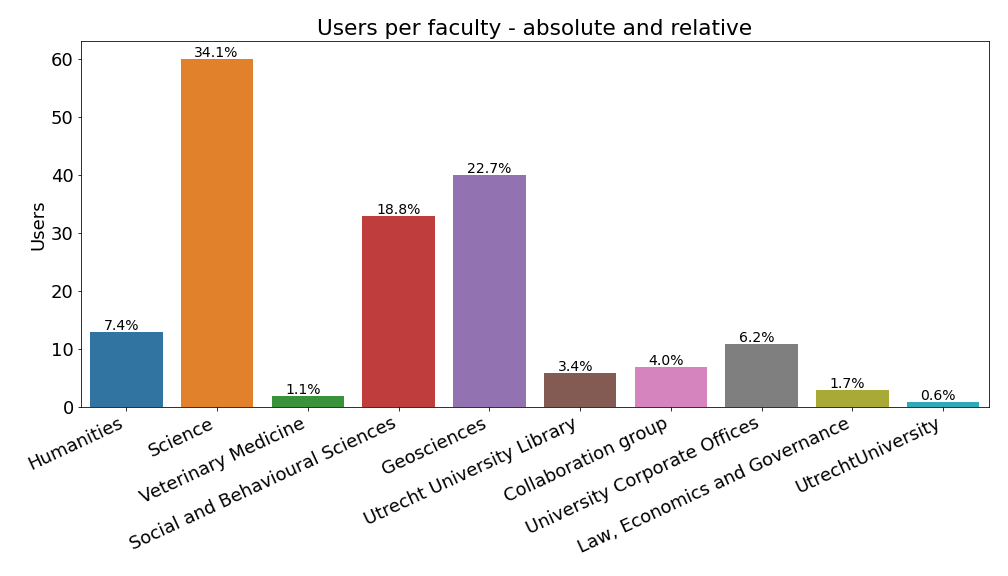
\includegraphics[scale=0.5]{figures_results/user_count.png}}
\caption{Number of users per faculty - both absolute and relative numbers. The y-axis shows the count, the number on top of a bar shows the percentage.
\label{fig:user_count}}
\end{figure}



The number of repositories per user per faculty can be seen in \autoref{fig:user_public_repos} as a swarm plot with an overlapping box plot. What can be seen is that most users have a small number of repositories. In contrast, only a few have a vast number of repositories. There is also no dominant faculty for the users with many repositories.


\autoref{fig:user_public_repos} shows the same plot with the user type instead of faculty. It shows that except for one user, it is usually an organization or collaboration group that has a large number of repositories. It also seems logical if this information is digested together with \autoref{fig:user_public_repos}. While there can be many users from a few faculties, there can naturally only be a few organizational-level users for each faculty.

\begin{figure}[h!]
\centerline{
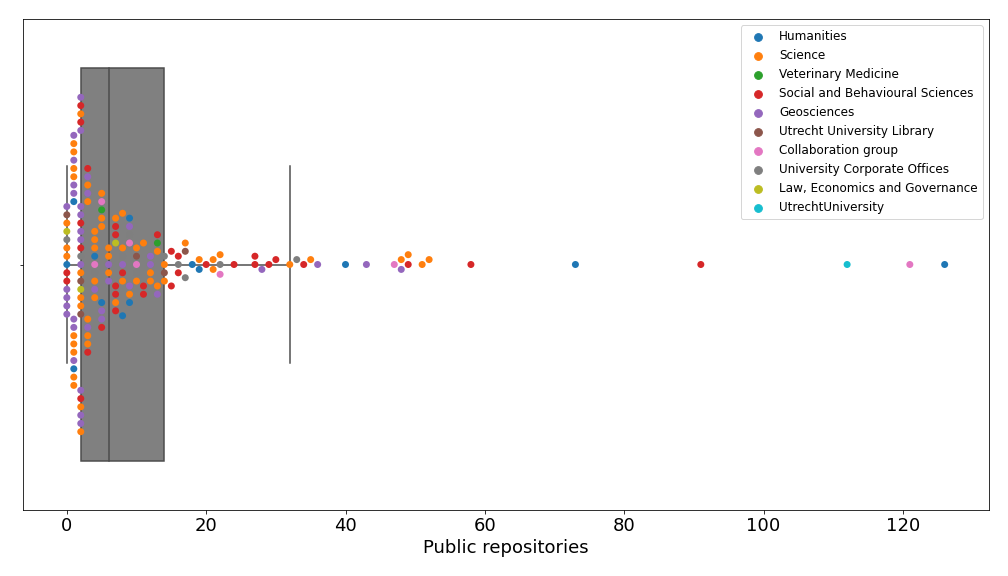
\includegraphics[scale=0.47]{figures_results/user_public_repos.png}}
\caption{Number of public repositories per faculty.
\label{fig:user_public_repos}}
\end{figure}


\begin{figure}[h!]
\centerline{
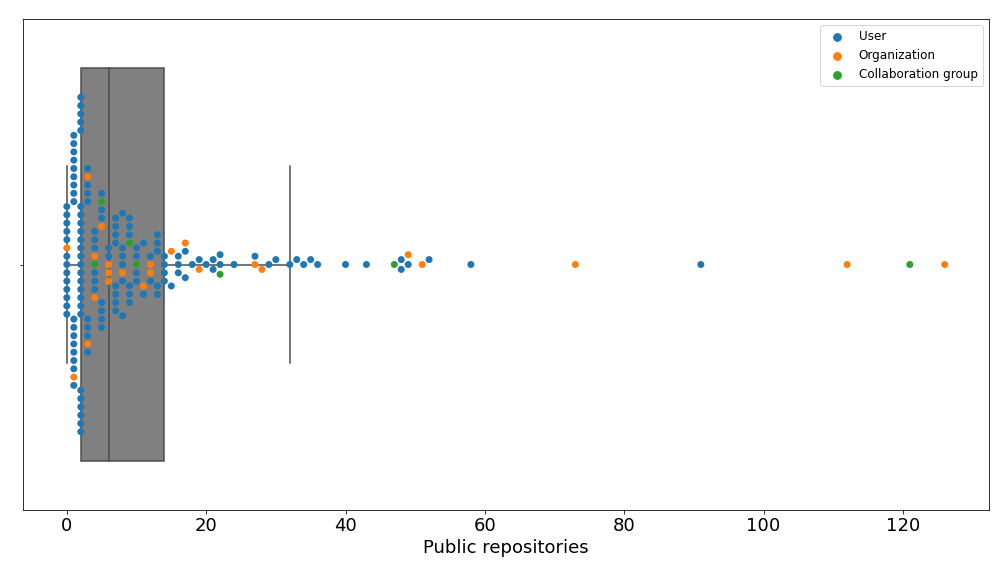
\includegraphics[scale=0.47]{figures_results/user_public_repos_usertype.png}}
\caption{Number of public repositories per user type.
\label{fig:user_public_repos_usertype}}
\end{figure}

\newpage

\autoref{tab:stats_users} shows the statistical measures of metrics for the collected users. The 25th quantile and median show that most users have a small number of followers and users they are following. The high values for skewness and kurtosis also indicate this. The number of repositories is similarly skewed but to a lesser extent, which the median also points towards. Additional box plots for number of followers and following can be seen in \autoref{app:user_plots}.


\begin{tabular}{lrrr}
\toprule
{} &  Public repositories &  Followers &  Following \\
\midrule
Minimum         &                 0.00 &       0.00 &       0.00 \\
25th percentile &                 2.00 &       0.00 &       0.00 \\
Mean            &                13.02 &      10.32 &       5.44 \\
Median          &                 6.00 &       2.00 &       1.00 \\
75th percentile &                14.00 &       9.00 &       4.00 \\
Maximum         &               126.00 &     210.00 &     103.00 \\
Skewness        &                 3.31 &       5.16 &       4.32 \\
Kurtosis        &                13.19 &      30.98 &      24.24 \\
\bottomrule
\end{tabular}




\section{Repository characteristics}
\label{sec:res_repos}
The number of collected research software repositories per faculty and repository type can be seen in \autoref{fig:heat_repo_count}. Interestingly, the \textit{Faculty of Law, Economics and Governance} has no open research-related repositories. We also see a low number of research-related repositories for the \textit{University Corporate Offices}, \textit{Utrecht University Library}, and the \textit{Faculty of Veterinary Medicine}.


\begin{figure}[h!]
\centerline{
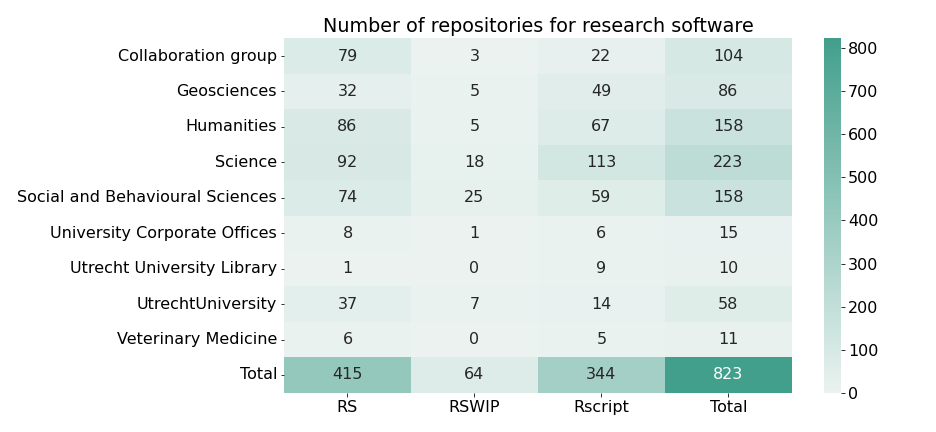
\includegraphics[scale=0.45]{figures_results/heatmap_repo_count.png}}
\vspace{-0.3cm}
\caption{Number of research software repositories grouped by faculty and repository type.
\label{fig:heat_repo_count}}
\end{figure}

Regarding non-research software, \autoref{fig:heat_repo_count_non_rs} shows that most non-research software is related to documentation, general non-research software, and workshops. This is logical, as most repositories within \textit{docs} and \textit{workshop} still relate to academia but are more relevant for archiving or educational purposes. Non-research software most often depicted either private projects or projects to get familiar with new programming languages, concepts, or algorithms.

\begin{figure}[h!]
\centerline{
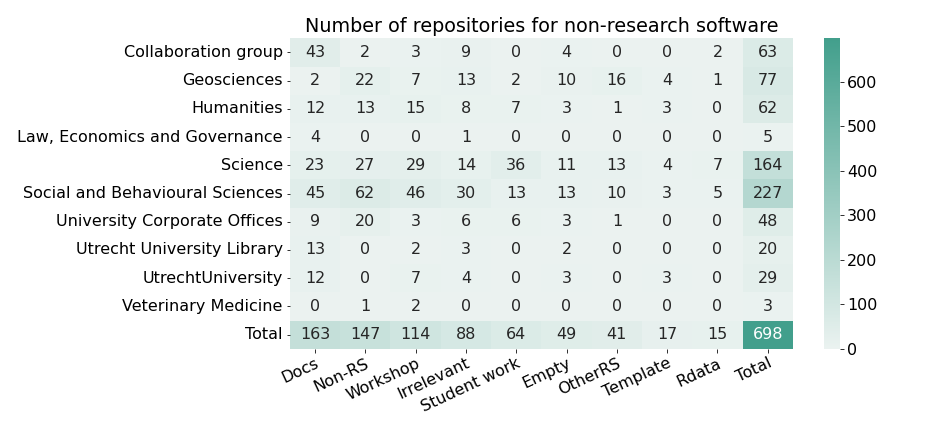
\includegraphics[scale=0.45]{figures_results/heatmap_repo_count_non_rs.png}}
\vspace{-0.3cm}
\caption{Number of non-research software repositories grouped by faculty and repository type.
\label{fig:heat_repo_count_non_rs}}
\end{figure}

\textit{University Corporate Offices} and \textit{Utrecht University Library} are support departments and will be grouped together with the group of \textit{UtrechtUniversity} for further analysis under the name of \textit{Support departments}. 
The faculties \textit{Veterinary Medicine} and \textit{Law, Economics and Governance} are excluded from further analysis due to the low amount of relevant repositories. 
However, this does not necessarily mean that there is no existing research software within these faculties. It could be that it is hosted on different platforms, that their findability is lacking, or that our search method is not well-adjusted to these faculties.
\textit{Collaboration group} is also excluded from further analysis, as discussed in \autoref{chap:method}. \textit{Social and Behavioral Sciences} will be shortened to \textit{Social Sciences} for readability purposes in the following analysis.


The final processed dataset on which the following analysis will be done can be seen in \autoref{fig:heat_repo_count_final}. All faculty groups now have a sufficient amount of research software repositories. The classes \textit{Total RS} and \textit{Total non-RS} are also relatively balanced, which is relevant for the classification.
\vspace{-0.2cm}

\begin{figure}[h!]
\centerline{
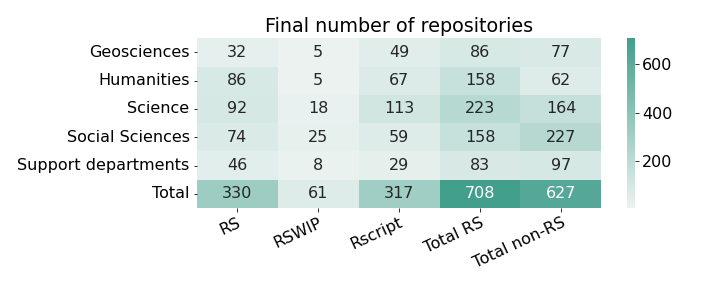
\includegraphics[scale=0.48]{figures_results/heatmap_repo_count_final.png}}
\vspace{-0.3cm}
\caption{Number of final research software repositories grouped by faculty and repository type. \textit{Total RS} aggregates the columns to the left, equivalent to previous Figures, while \textit{total non-rs} additionally shows the number of repositories that are considered non-research software. 
\label{fig:heat_repo_count_final}}
\end{figure}

\newpage

\autoref{fig:stats_histograms} shows the histograms for all metrics split into the two classes \textit{research software} and \textit{non-research software}. We can see that the data are heavily long-tailed for both classes. There are a few repositories that have much higher metrics than most of the other ones. Except for number of contributors, research software usually has more large values than non-research software. 
Histograms with only research software and a heatmap of the most common topics can be seen in \autoref{app:repo_plots}.


\begin{figure}[h!]
\centerline{
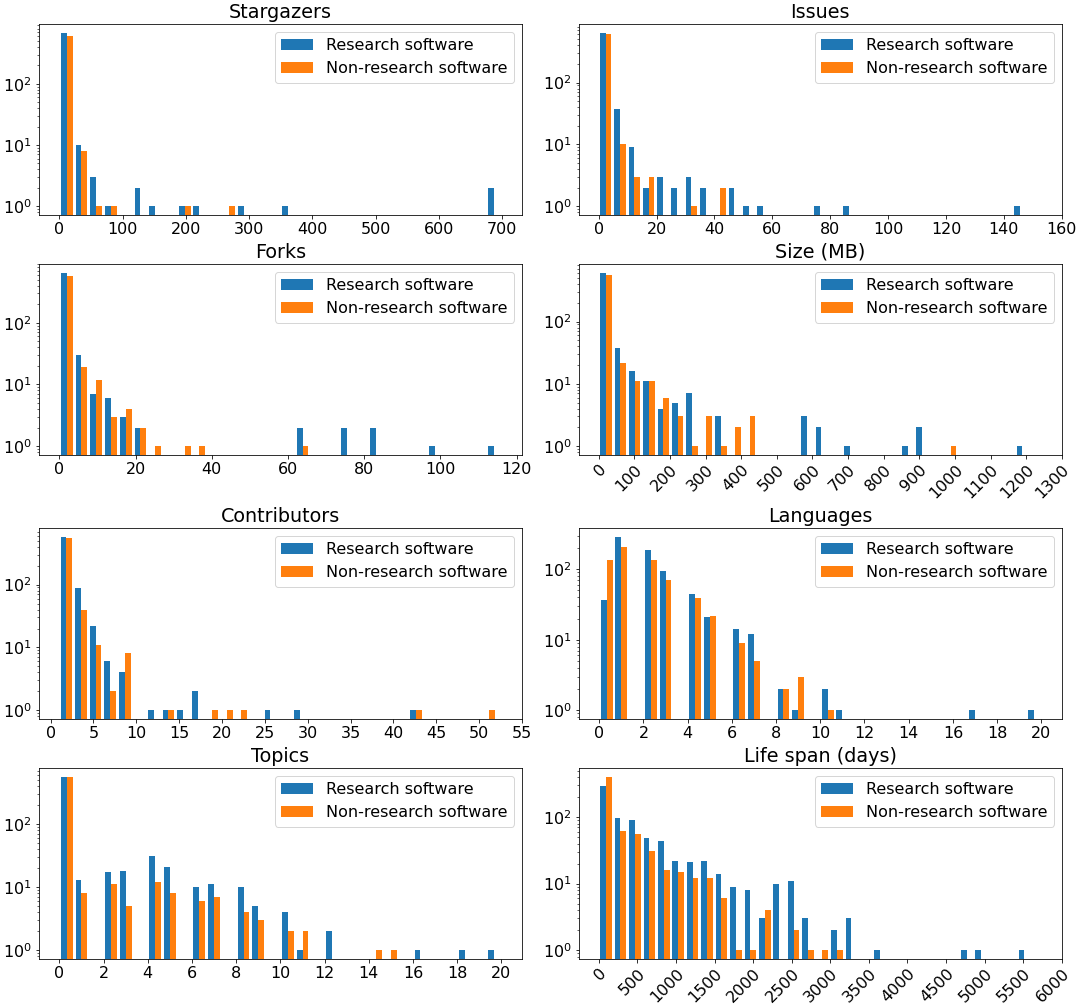
\includegraphics[scale=0.54]{figures_results/stats_histograms.png}}
\caption{Histograms for metrics categorized by research software vs. non-research software. The y-axis is log-scaled.
\label{fig:stats_histograms}}
\end{figure}

\autoref{fig:heatmap_numeric_variables} shows the heatmaps for all averages of metrics collected for the repositories. This shows us that the averages are usually the highest for the repository type of research software. The number of languages and life span are roughly equal across the faculties. Geosciences have the highest average for open issues and the lowest average for contributors. Humanities have the lowest average for stargazers, forks, size, and topics often by a substantial amount. Science has the highest average for size and the lowest average for open issues. 
This is followed closely by Social Sciences, which are otherwise in-between other averages except for the number of languages. This might indicate that they primarily use only a few programming languages. The Support department has the highest average of stargazers by far, as well as forks, contributors, and topics.

\begin{figure}[tbph!]
\centerline{
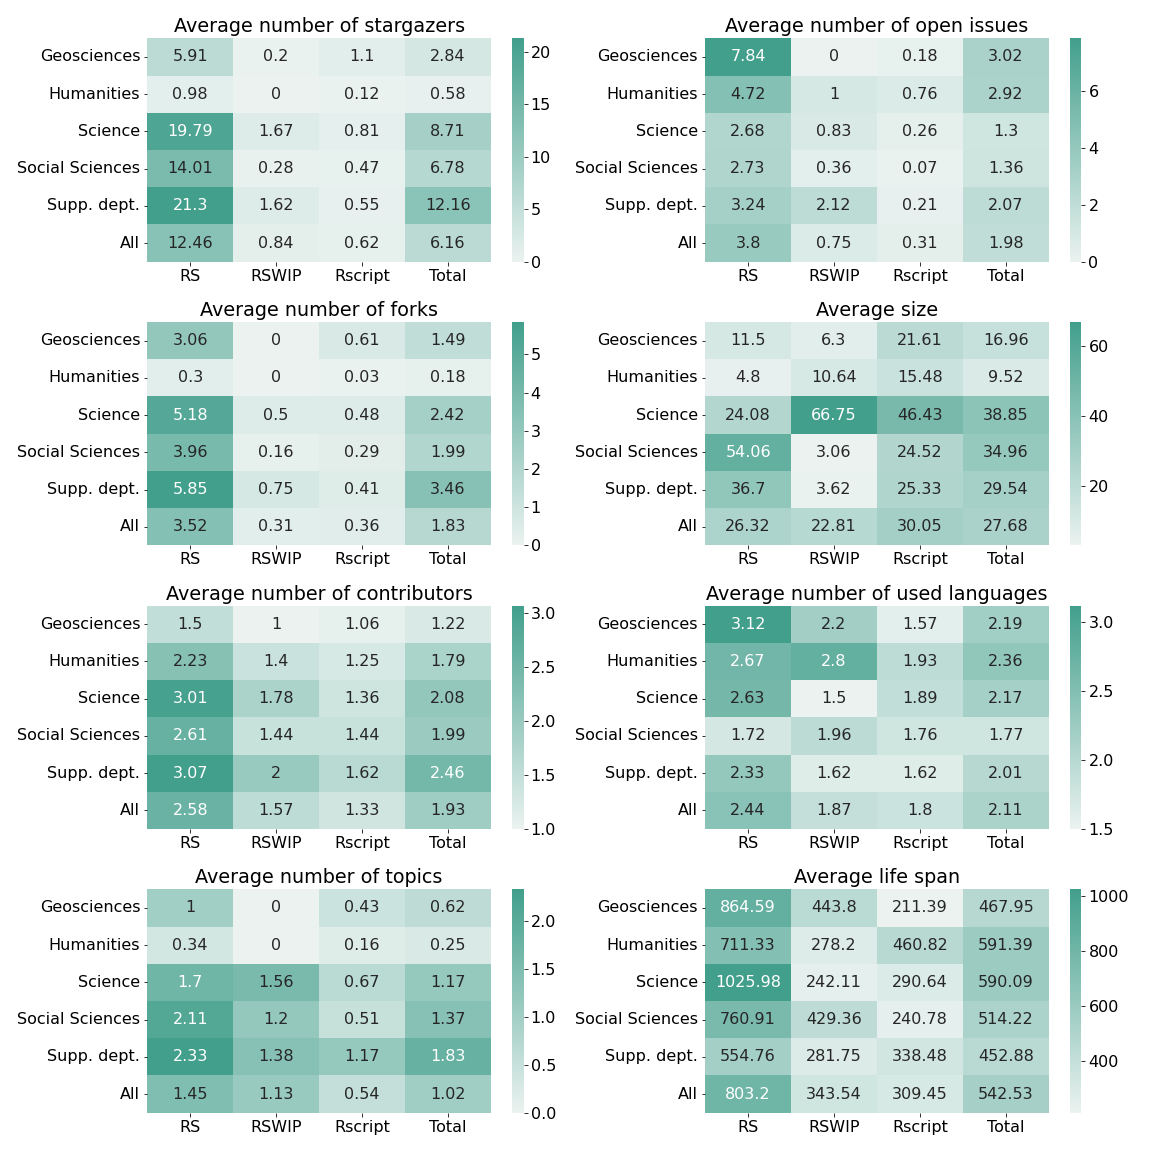
\includegraphics[scale=0.5]{figures_results/heatmap_numeric_variables.png}}
\caption{Heatmaps for all metrics grouped by faculty and repository type. \textit{All} and \textit{Total} refer to the average across all research software repositories. Therefore, these rows and columns do not equal the average across different rows and columns, since it also takes the number of repositories in each cell into account. This will also be the case for the following Figures.
\label{fig:heatmap_numeric_variables}}
\end{figure}

% LICENSES %
% LICENSES %
% LICENSES %


\autoref{tab:highest_license} shows the highest occurring license for each faculty across the different repository types. There are a few things to note here: Science is the only faculty where Apache 2.0 appears, while every other faculty has a GPL license at the top. Each faculty has an MIT license at the top. Clearly, the dominating licenses are MIT and GPLv2/GPLv3. 

\begin{table}
\centering
\caption{Highest occurring license per faculty per repository type.}
\label{tab:highest_license}
\begin{tabular}{lccc}
\toprule
repo\_type &          RS &  RSWIP &     Rscript \\
faculty             &             &        &             \\
\midrule
Geosciences         &       GPLv3 &    MIT &  GPLv3, MIT \\
Humanities          &  GPLv2, MIT &  Other &       GPLv2 \\
Science             &  Apache 2.0 &    MIT &         MIT \\
Social Sciences     &       Other &  GPLv3 &  GPLv3, MIT \\
Support departments &         MIT &  GPLv3 &         MIT \\
\bottomrule
\end{tabular}
\end{table}


\newpage
\newpage

We can take a deeper look into the license usage in \autoref{fig:heatmap_licenses}. This shows the license percentage for each faculty. What this also reveals is the percentage of no license usage. If we would also consider no license, this would be the dominating license usage for all faculties except the Support department. Most notable is Geosciences, with 57\% of repositories having no license, which is 22 percentage points more than the following faculty, Humanities. Social Sciences have the least amount of unlicensed software. As we have seen from \autoref{tab:highest_license}, the most common licenses are MIT and GPLv3. The licenses that follow afterwards are predominantly used by only one of the faculties.



\begin{figure}[tbph!]
\centerline{
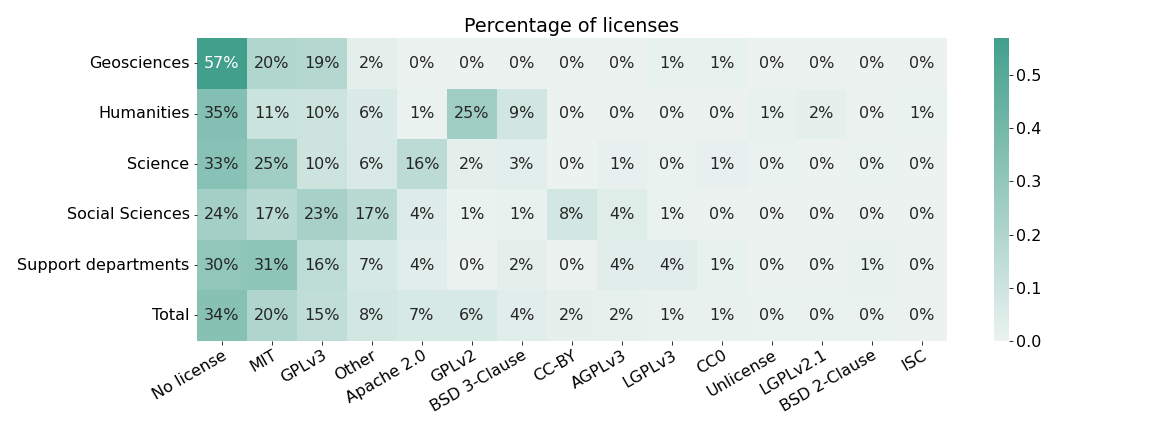
\includegraphics[scale=0.5]{figures_results/heatmap_licenses.png}}
\caption{Heatmap grouped by faculty for percentage of licenses sorted from left to right by total percentage. The percentages sum up to 100\% across rows.
\label{fig:heatmap_licenses}}
\end{figure}

% LANGUAGES %
% LANGUAGES %
% LANGUAGES %

\autoref{tab:highest_language} shows the highest occurring language for each faculty across the different repository types. As expected, Python and R are dominating most categories. Science and Social Sciences stand out, with Python and R as the top language across all repository types, respectively. The only outliers to this are RSWIP and Rscript for Geosciences and Humanities. The category RSWIP for Geosciences and Humanities only have five repositories each, limiting the conclusions that can be drawn from this. That MATLAB would be common for Geosciences in Rscript is plausible, as it is widely used where matrix manipulation is necessary, like processing of images. Shell is the most common language for Humanities in Rscript since the programming language Zep is often used here and is not detected by GitHub. This concerns many repositories from the \acrfull{uilotslab}.


\begin{table}
\centering
\caption{Highest occurring language per faculty per repository type.}
\label{tab:highest_language}
\begin{tabular}{lccc}
\toprule
repo\_type &      RS &                              RSWIP & Rscript \\
faculty             &         &                                    &         \\
\midrule
Geosciences         &  Python &  JavaScript, MATLAB, Python, Shell &  MATLAB \\
Humanities          &  Python &                         JavaScript &   Shell \\
Science             &  Python &                             Python &  Python \\
Social Sciences     &       R &                                  R &       R \\
Support departments &  Python &                                  R &       R \\
\bottomrule
\end{tabular}
\end{table}


\autoref{fig:heatmap_languages_tenplus} shows all languages that were the top language in at least ten repositories. This confirms again that Social Sciences use mainly R for their research, while Python is most common for all other faculties. We can see a similar pattern to the licenses. After the first two top languages, the next ones are again predominantly used by only one of the faculties. The column \textit{No language} is a special case where no language could be detected. In some cases, the contributors omitted the file extension, which GitHub uses to detect the languages.

\begin{figure}[h!]
\centerline{
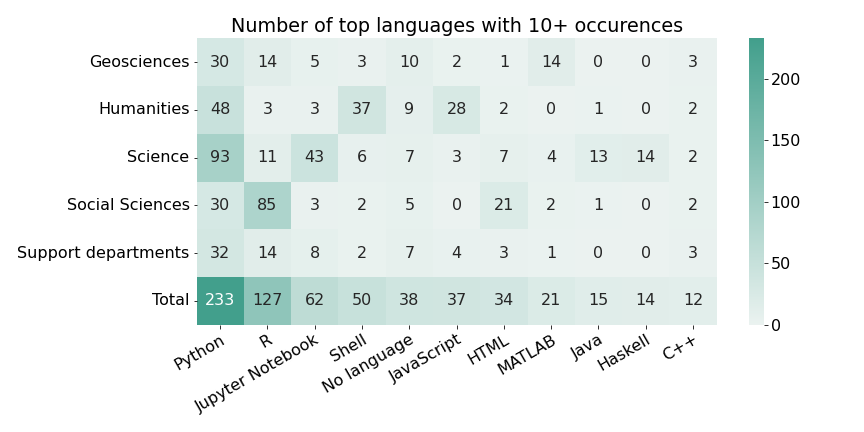
\includegraphics[scale=0.5]{figures_results/heatmap_languages_tenplus.png}}
\caption{Heatmap grouped by faculty for number of top languages sorted from left to right. Only languages with more than 10 total occurrences as top language are shown.
\label{fig:heatmap_languages_tenplus}}
\end{figure}

\autoref{fig:heatmap_languages_percentage} shows all languages that appeared in at least 10\% of the repositories in a faculty. This considers all detected languages in a repository, not only the top language. While Jupyter Notebooks are often the dominant language, as \autoref{fig:heatmap_languages_tenplus} shows, they are present in only a small amount of repositories. Shell also moved up by one spot; all faculties except for Social Sciences have used Shell in at least 20\% of their repositories. This further indicates that Social Sciences might behave differently from other faculties regarding language usage. 
There is also a clear difference in language usage between Social Sciences and the other faculties, as R is used in 72\% of repositories within that faculty, while the others barely use it. They have a strong preference for Python, which is present in about 50\% of their repositories. Social Sciences, on the other hand, has Python present in only about 25\% of the repositories.

\vspace{-0.2cm}
\begin{figure}[h!]
\centerline{
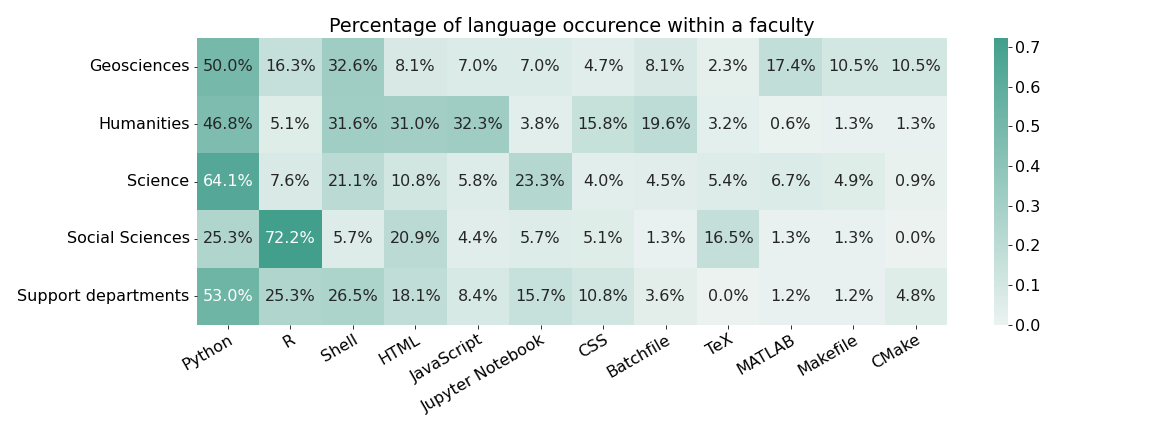
\includegraphics[scale=0.5]{figures_results/heatmap_languages_percentage.png}}
\caption{Heatmap grouped by faculty for percentage of language occurence sorted from left to right based on added percentage per column. This shows all languages that occurred in at least 10\% of the repositories within a faculty. The percentage represents how many repositories within a faculty used the mentioned language. As such, the percentage does not sum up to 100 across the columns or rows. If all languages within a faculty appeared in all repositories, they would all have 100\%.
\label{fig:heatmap_languages_percentage}}
\end{figure}

% CORRELATION %
% CORRELATION %
% CORRELATION %

\vspace{-0.3cm}
\autoref{fig:heatmap_correlation_numeric} shows the correlation matrix for metrics. We can see a strong correlation between the number of stargazers and forks, between the number of forks and contributors, and a moderate relationship between the number of stargazers with contributors or topics. Forking is usually done to contribute to a repository, and users usually contribute to repositories they starred. A moderate relationship can be seen for number of issues with contributors and languages and contributors with life span. This seems logical, as contributors often communicate via issues, and more contributors allow for a broader range of skills and used languages. They also facilitate software maintenance over longer periods.

\begin{figure}[tbph!]
\centerline{
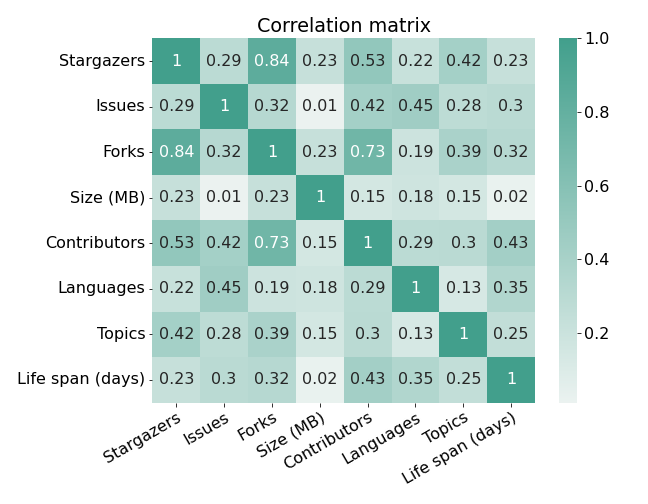
\includegraphics[scale=0.5]{figures_results/heatmap_correlation_numeric.png}}
\caption{Correlation matrix for all metrics.
\vspace{-0.3cm}
\label{fig:heatmap_correlation_numeric}}
\end{figure}
\vspace{-0.3cm}

Descriptive statistics of all metrics can be seen in \autoref{tab:all_faculties}. The skewness and kurtosis show us that all metrics are heavily skewed and long-tailed, albeit to different degrees. The statistics per faculty can be seen in \autoref{app:stats_faculty}. These show us that the median for all metrics except life span is relatively similar across all faculties.
% TODO: write more?

\begin{table}
\centering
\caption{Descriptive statistics of numeric variables for all faculties}
\label{tab:all_faculties}
\begin{tabular}{lcccccccc}
\toprule
{} &  Stargazers &  Issues &   Forks &     Size &  Contributors &  Languages &  Topics &  Life span \\
\midrule
Minimum         &        0.00 &    0.00 &    0.00 &     0.00 &          1.00 &       0.00 &    0.00 &       0.00 \\
25th percentile &        0.00 &    0.00 &    0.00 &     0.07 &          1.00 &       1.00 &    0.00 &      33.00 \\
Mean            &        6.16 &    1.98 &    1.83 &    27.68 &          1.93 &       2.11 &    1.02 &     542.53 \\
Median          &        0.00 &    0.00 &    0.00 &     0.68 &          1.00 &       2.00 &    0.00 &     295.50 \\
75th percentile &        1.25 &    1.00 &    1.00 &     7.65 &          2.00 &       3.00 &    0.00 &     737.75 \\
Maximum         &      699.00 &  148.00 &  116.00 &  1209.65 &         42.00 &      20.00 &   20.00 &    5609.00 \\
Skewness        &       12.95 &    9.85 &    8.96 &     6.84 &          8.59 &       3.36 &    3.15 &       2.41 \\
Kurtosis        &      189.27 &  127.60 &   87.08 &    55.84 &        101.50 &      21.87 &   12.73 &       8.28 \\
\bottomrule
\end{tabular}
\end{table}





\newpage
\section{\acrshort{fair} variables}
\label{sec:res_fair}

\autoref{fig:jaccard} shows the Jaccard similarity of all boolean \acrshort{fair} variables. The Jaccard similarity between any variable with \textit{repository open} approximately equals the percentage of true occurrences of the concerned variable since \textit{repository open} is true for nearly all repositories. This shows that the three howfairis variables related to \textit{registry, citation, and checklist} are found only in a small number of repositories, while the newly proposed ones are more frequent. We can also see that the correlation between the howfairis variables is not relatively high, except for the two variables related to registry and checklist.
From the first and second rows, we can see that except for the variable \textit{correct vcs usage} and \textit{repository active}, all \acrshort{fair} variables are more frequent or at least equal in case the repository has a license. \textit{Is registered} has a higher similarity with \textit{has contrib. guidelines}. Since research software that is registered is often developed by multiple people, it seems logical that these kinds of research software should have more guidelines for contribution. A similar logical argument can be made for the \textit{has citation} and \textit{version identifiable} since the Zenodo citation integration uses release tags. 268 out of 337 tags, or roughly 80\% of repositories with tags, were correctly using identifiable versioning. 

\begin{figure}[h!]
\centerline{
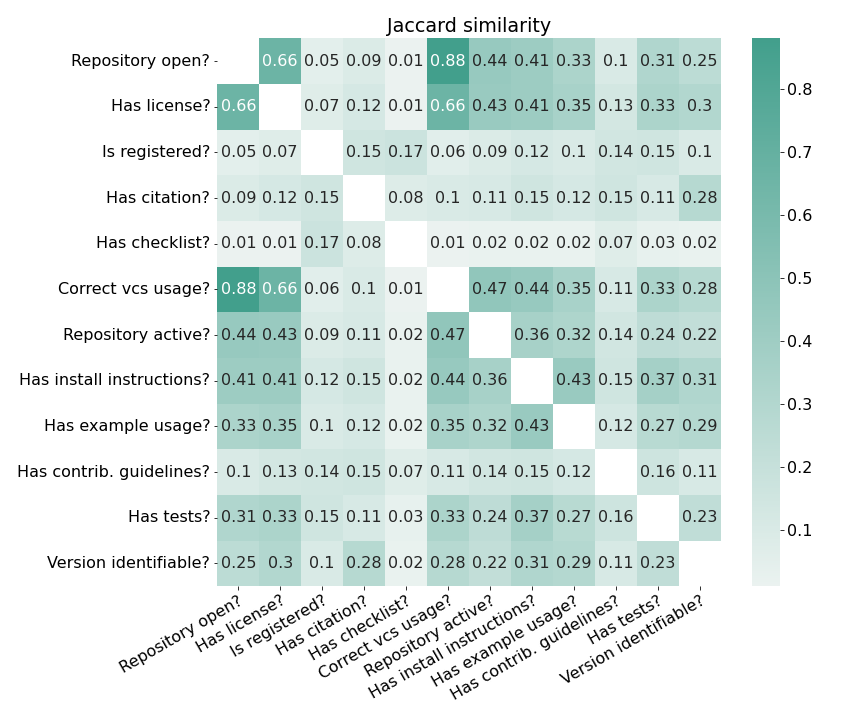
\includegraphics[scale=0.5]{figures_results/heatmap_jaccard_similarity.png}}
\caption{Jaccard similarity for all boolean \acrshort{fair} variables.
\label{fig:jaccard}}
\end{figure}

\autoref{fig:heatmap_fair_booleans} shows the heatmaps for the average percentage of each boolean \acrshort{fair} variable per faculty. The upper plot shows the averages for research software, while the lower one shows averages for non-research software. We can immediately see from this that every \acrshort{fair} variable has a higher percentage for research software than for non-research software. Large absolute increases can be seen in \textit{has license, correct vcs usage, has install instructions, has tests, and version identifiable}. 
Social Sciences has the highest percentage of licenses across both classes for research software, while Geosciences has the lowest percentage. Social Sciences also have a high percentage of repositories that are registered, have citation enabled, or contain a checklist, compared to other faculties. Geosciences have the lowest average percentage of correct vcs usage, meaning that more than 20\% of the research software repositories had only commits within a single day. Social Sciences and Support departments have a high percentage of active repositories, while other faculties are generally less active. Support departments, by far, have the highest percentage of install instructions and usage examples. For contribution guidelines, Social Sciences and Support departments again are around the same high percentage, while other faculties have only a minuscule amount. Geosciences and Humanities, the two faculties with the lowest percentage, are also the ones with the least amount of contributors. Interestingly, the Science faculty has the least amount of tests and identifiable versions on average.

% TODO: --> followup for discussion, Geo might need more support for actual use of GitHub and its features (licensing, version control usage)
\begin{figure}[h!]
\centerline{
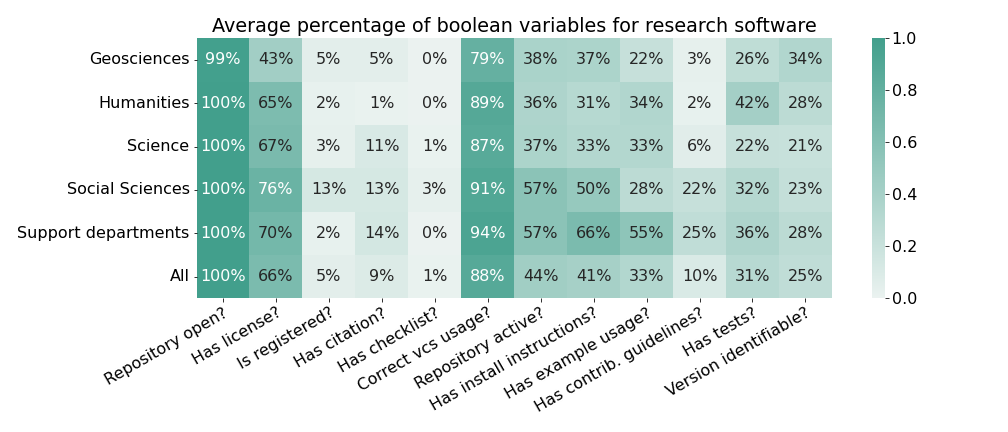
\includegraphics[scale=0.53]{figures_results/heatmap_fair_booleans.png}}
\vspace{-0.5cm}
\centerline{
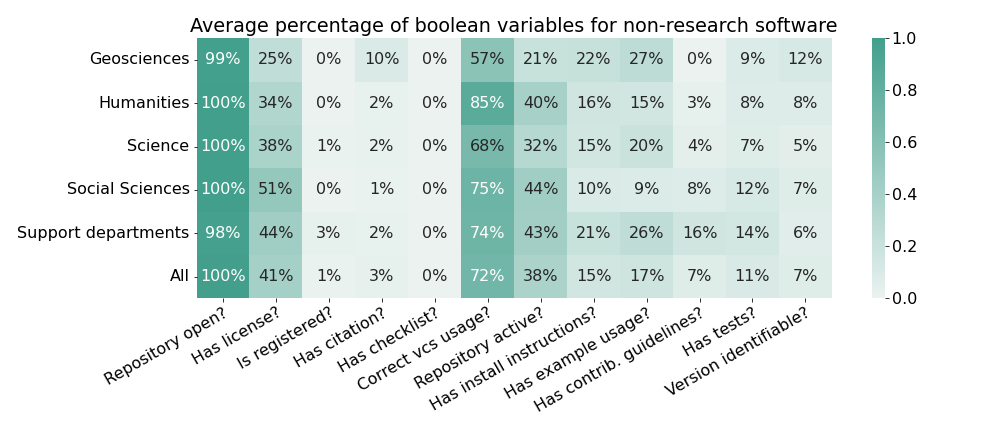
\includegraphics[scale=0.53]{figures_results/heatmap_fair_booleans_non_rs.png}}

\caption{Heatmaps for all boolean \acrshort{fair} variables grouped by faculty. The upper heatmap shows the averages for research software, while the lower one shows the averages for non-research software.
\label{fig:heatmap_fair_booleans}}
\end{figure}

\newpage
\autoref{fig:fair_score} shows the \acrshort{fair} score calculated as the sum of all boolean \acrshort{fair} variables for each repository. We can see that \textit{Rscripts} have a lower sum average than both \textit{RS} and \textit{RSWIP}. We can also see that Social Sciences and Support departments receive relatively high scores compared to the other faculties, with Geosciences having the lowest average score.

\begin{figure}[tbph!]
\centerline{
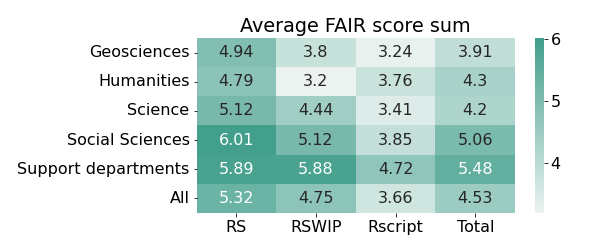
\includegraphics[scale=0.5]{figures_results/heatmap_fair_score.png}}
\vspace{-0.3cm}
\caption{FAIR score of boolean \acrshort{fair} variables grouped by faculty and repository type. The score for each repository is calculated as the number of true \acrshort{fair} variables, which are all booleans. 
\label{fig:fair_score}}
\end{figure}


\vspace{-0.2cm}
\section{Statistical tests}
\label{sec:stattests}
In order to statistically determine whether there are different characteristics in the metrics between faculties, we performed Kruskal-Wallis tests for each metric, followed by post hoc test analyses via Dunn's test. The results of the Kruskal-Wallis tests can be seen in \autoref{tab:kruskal_wallis}. All metrics have significant differences except for life span. \autoref{fig:stats_dunn_pvalues} shows the post hoc test results. A p-value smaller than 0.05 indicates that the two groups come from a significantly different distribution. Overall, we can see that Science, Social Sciences and Support department are not too different, as they only have significant p-values within \textit{open issues} and \textit{topics}. Geosciences and Humanities, however, are frequently dissimilar to other faculties. Geosciences is the only different faculty for the number of contributors compared to all other ones.

\begin{table}
\centering
\caption{Kruskal-Wallis test results}
\label{tab:kruskal_wallis}
\begin{tabular}{lcc}
\toprule
          Variable &      p-value &  Significant? \\
\midrule
  stargazers\_count & 1.247649e-08 &          True \\
       open\_issues & 6.513571e-06 &          True \\
             forks & 1.301400e-09 &          True \\
              size & 3.112421e-04 &          True \\
contributors\_count & 3.651742e-05 &          True \\
   languages\_count & 1.750939e-02 &          True \\
      topics\_count & 1.668033e-11 &          True \\
         life\_span & 2.769494e-01 &         False \\
\bottomrule
\end{tabular}
\end{table}



\begin{figure}[h!]
\centerline{
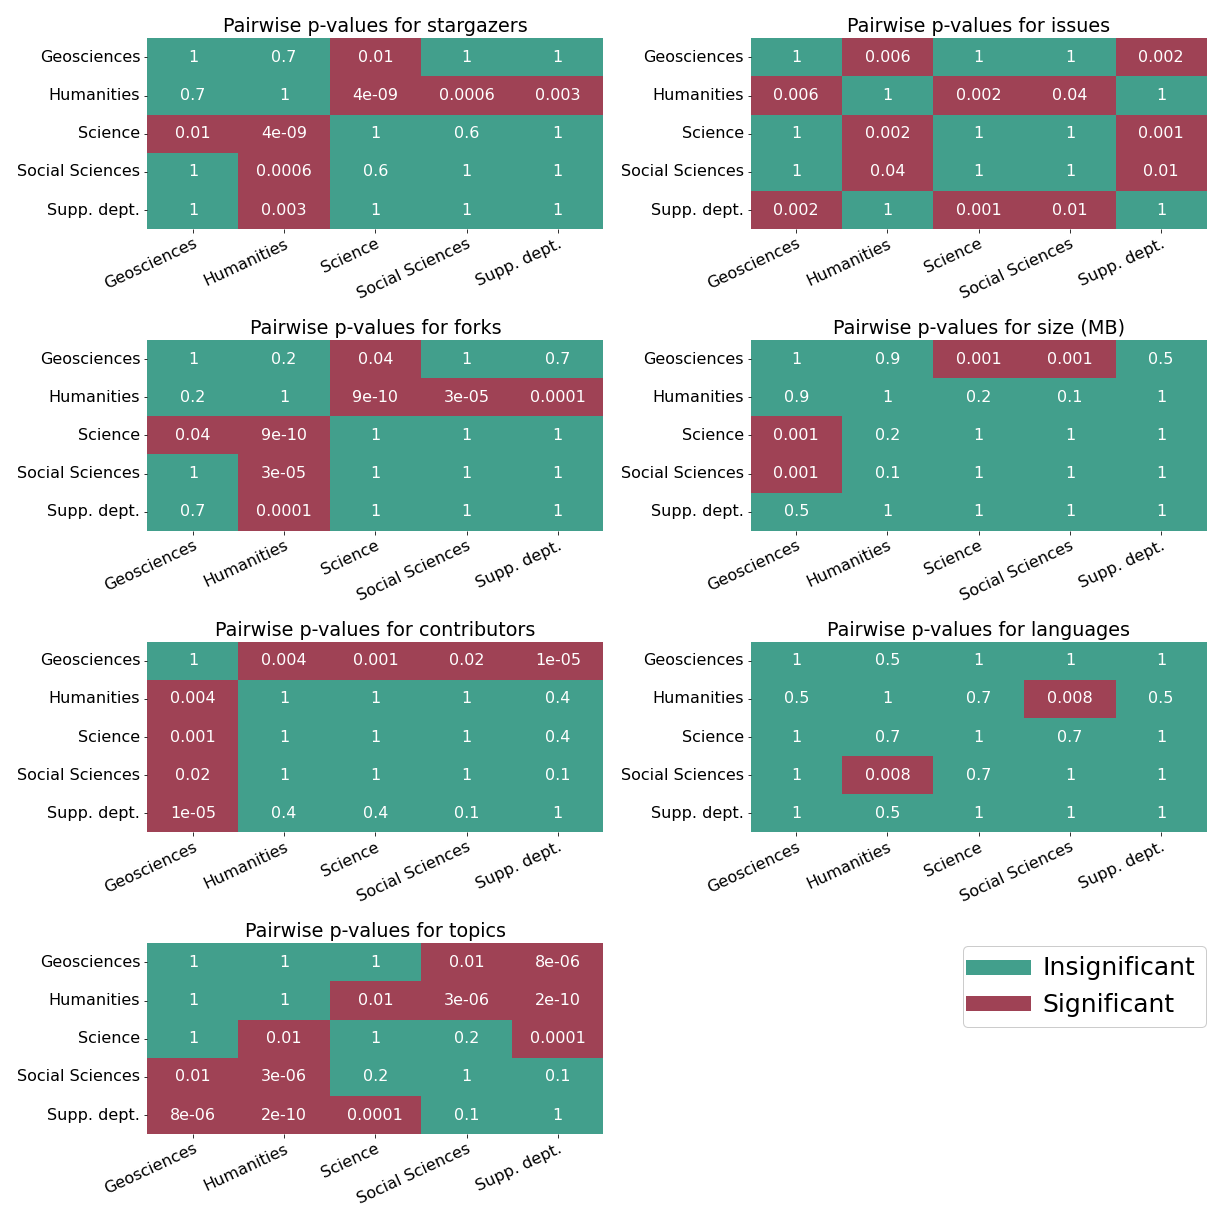
\includegraphics[scale=0.47]{figures_results/stats_dunn_pvalues.png}}
\caption{Dunn's test results for each variable.
\label{fig:stats_dunn_pvalues}}
\end{figure}


\newpage
\section{Research software classification}
\label{sec:classification}
We predict whether a repository is considered research software or not based on two trained models and a chance prediction.
\autoref{fig:stats_confusion_matrices} shows the confusion matrices for both model predictions and chance predictions for the research software classification. We can see from this that random forest performed better than logistic regression since there are fewer false negatives and false positives. 

\begin{figure}[h!]
% \vspace*{-1cm}
\centerline{
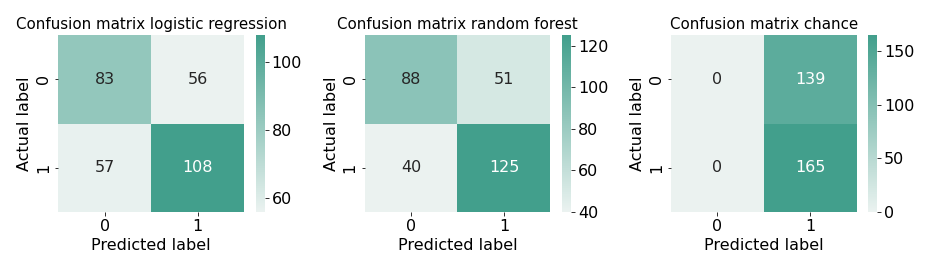
\includegraphics[scale=0.5]{figures_results/stats_confusion_matrices.png}}
\caption{Confusion matrices for logistic regression, random forest, and chance.
\label{fig:stats_confusion_matrices}}
\end{figure}



Based on the confusion matrix, further performance measures are calculated in \autoref{fig:stats_barplot_scores}, which shows the performance measures for both model and chance predictions. Both models outperform the chance classification in accuracy and precision. Random forest achieves a higher score in all performance measures than logistic regression and chance except for recall, which is expected. A random forest can better utilize complex variables than a logistic regression, where an increase in a variable value always increases or decreases the probability of a positive classification. This shows that the used variables improve classification compared to a chance classifier, that we can improve research software identification accuracy by 16 percentage points, and that a random forest is more suitable than logistic regression for this classification task.

\begin{figure}[h!]
% \vspace*{-1cm}
\centerline{
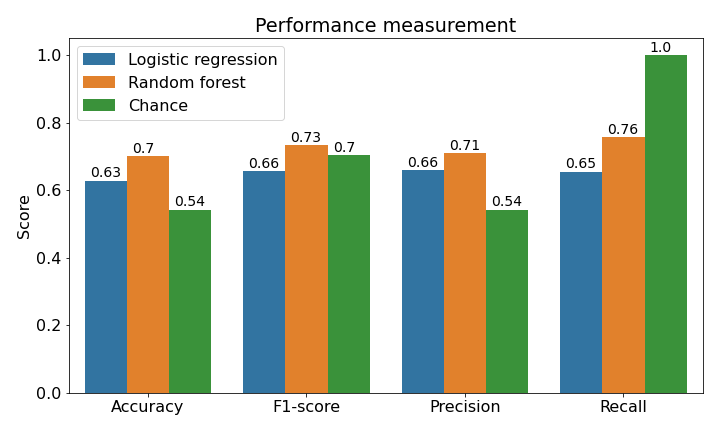
\includegraphics[scale=0.5]{figures_results/stats_barplot_scores.png}}
\caption{Performance measures of logistic regression, random forest, and chance.
\label{fig:stats_barplot_scores}}
\end{figure}

\newpage
\autoref{fig:stats_feature_importance_logit} shows the feature importance for the logistic regression model measured by the strength of the coefficients. The number of contributors has the highest effect, followed by life span and issues. After these, there is a steep decrease in the coefficient strength. 

\autoref{fig:stats_feature_importance_rf} shows the permutation feature importance for the random forest model. Since the performance of this model was better than for logistic regression, we assume these feature importances to be more relevant. Life span is also an important feature for this model, with a 5.1\% mean accuracy decrease, but the other top features differ. There is also a more gradual decrease in importance, as the variable languages follows with a 4.5\% mean accuracy decrease. The following features \textit{size, has install instructions, has license, has tests} all have a mean accuracy decrease of more than 2\%. 




\begin{figure}[h!]
\centerline{
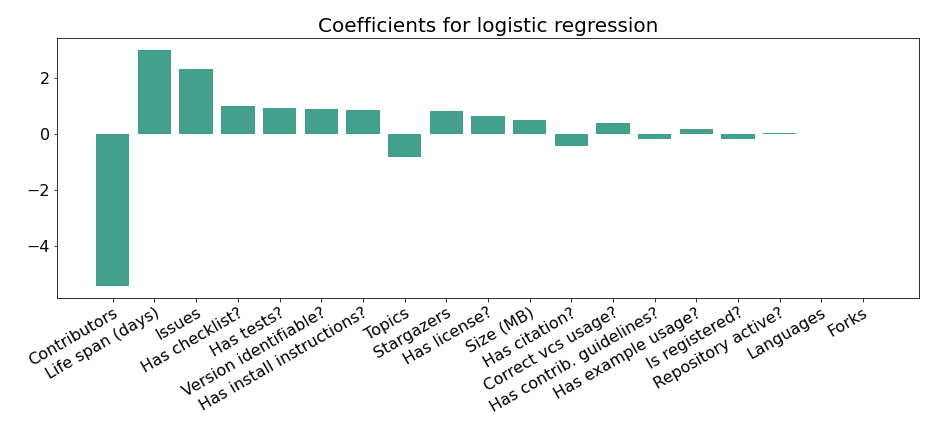
\includegraphics[scale=0.5]{figures_results/stats_feature_importance_logit.png}}
\caption{Feature importance for logistic regression shows the coefficients for each feature. A negative value indicates that an increase in that variable leads to a higher chance that the classified repository is not research software. The feature importance should therefore be viewed as an absolute value.
\label{fig:stats_feature_importance_logit}}
\centerline{
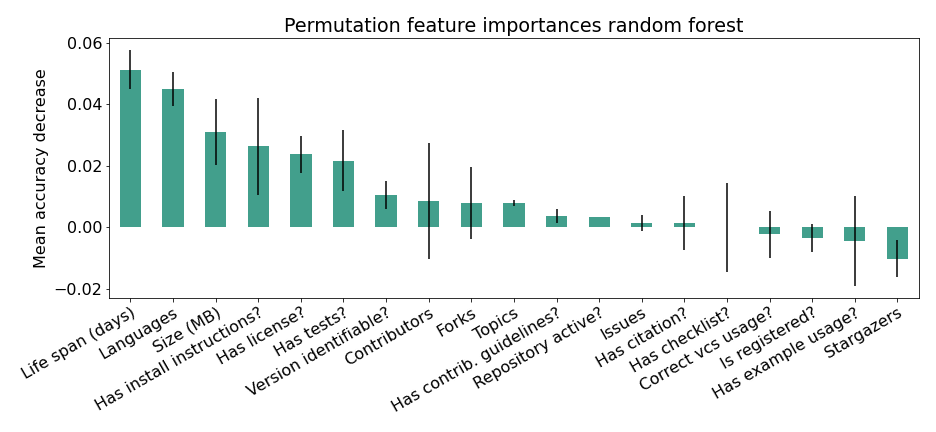
\includegraphics[scale=0.5]{figures_results/stats_feature_importance_forest.png}}
\caption{Feature importance for random forest. The y-axis shows by how many accuracy percentage points the random forest would perform worse if that feature would be removed. A negative importance can be interpreted that this is an irrelevant feature.
% https://www.kaggle.com/code/dansbecker/permutation-importance
\label{fig:stats_feature_importance_rf}}
\end{figure}